\section{Resultados}

% Sistema 1: Conway 2D

\begin{frame}{Conway 2D}
    \begin{multicols}{2}
        {
            $border = (0, 0) \times (100, 100)$

            $condition = \text{MOORE}$

            $r = 1$

            $shouldKeepAlive = [2, 3]$

            $shouldRevive = [3]$

            $initialDomainProportion = 0.16$

            $initialLiveCellsProportion = 0.60$
        }

        {\begin{figure}[H]
             \centering
             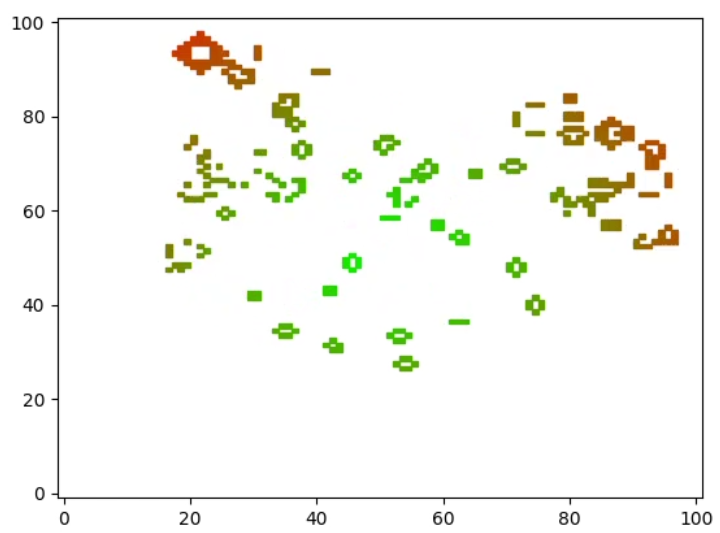
\includegraphics[width=1\linewidth]{pic/conway2d/thumbnail_i60}
             \captionsetup{font={scriptsize}}
             \captionsetup{labelformat=empty}
             \caption{Link al video: https://youtu.be/1HHKAB-ZeT4}
             \label{fig:conway2d:thumbnail}
        \end{figure}}
    \end{multicols}
\end{frame}

\begin{frame}{Conway 2D}
    \textbf{Cantidad de celdas vivas en función del tiempo}
    \begin{multicols}{2}
        {
            \begin{figure}[H]
                \centering
                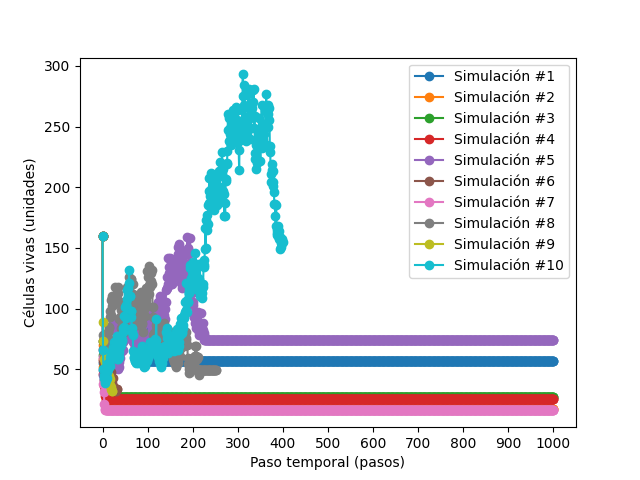
\includegraphics[width=0.8\linewidth]{pic/conway2d/size_i10}
                \text{$initialLiveCellsProportion = 0.10$}
                \label{fig:conway2d:size:i10}
            \end{figure}
        }


        {
            \begin{figure}[H]
                \centering
                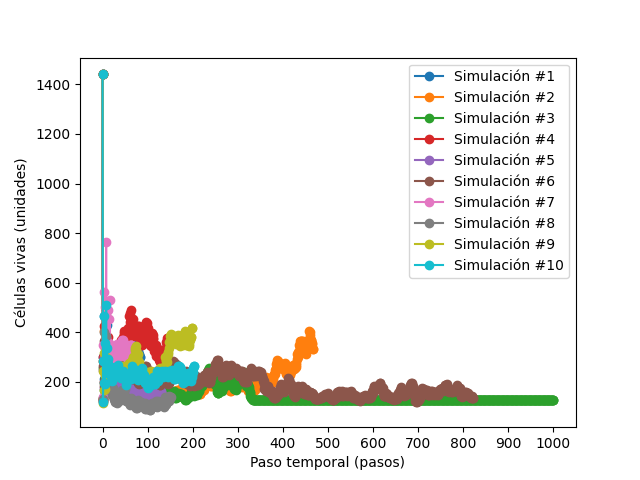
\includegraphics[width=0.8\linewidth]{pic/conway2d/size_i90}
                \text{$initialLiveCellsProportion = 0.90$}
                \label{fig:conway2d:size:i90}
            \end{figure}
        }
    \end{multicols}
\end{frame}

\begin{frame}{Conway 2D}
    \textbf{Observable: Cantidad de celdas vivas en el equilibrio}
    \begin{figure}[H]
        \centering
        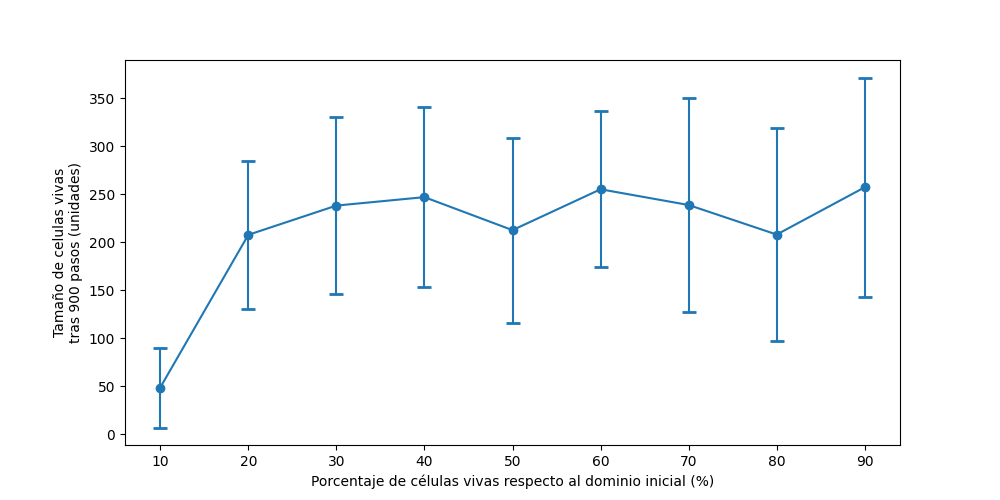
\includegraphics[width=0.8\linewidth]{pic/conway2d/size_vs_input}
        \label{fig:conway2d:size:density}
    \end{figure}
\end{frame}

\begin{frame}{Conway 2D}
    \textbf{Observable: Variación de la cantidad de celdas vivas}
    \begin{figure}[H]
        \centering
        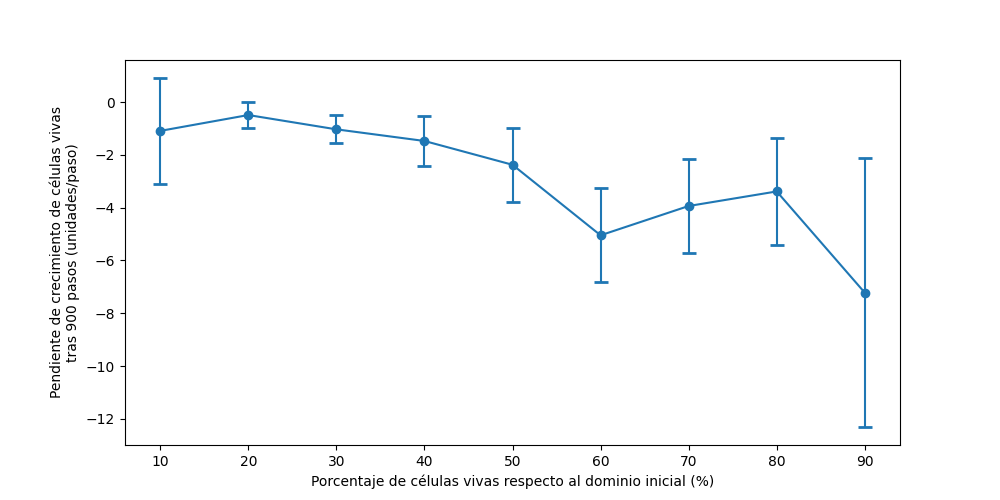
\includegraphics[width=0.8\linewidth]{pic/conway2d/size_slope_vs_input}
        \label{fig:conway2d:size_slope:density}
    \end{figure}
\end{frame}

\begin{frame}{Conway 2D}
    \textbf{Distancia de la celda viva más lejana al centro en función del tiempo}
    \begin{multicols}{2}
        {
            \begin{figure}[H]
                \centering
                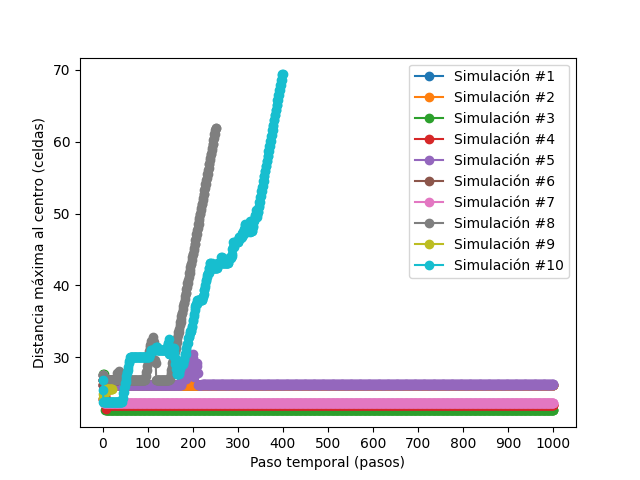
\includegraphics[width=0.8\linewidth]{pic/conway2d/distance_i10}
                \text{$initialLiveCellsProportion = 0.10$}
                \label{fig:conway2d:distance:i10}
            \end{figure}
        }


        {
            \begin{figure}[H]
                \centering
                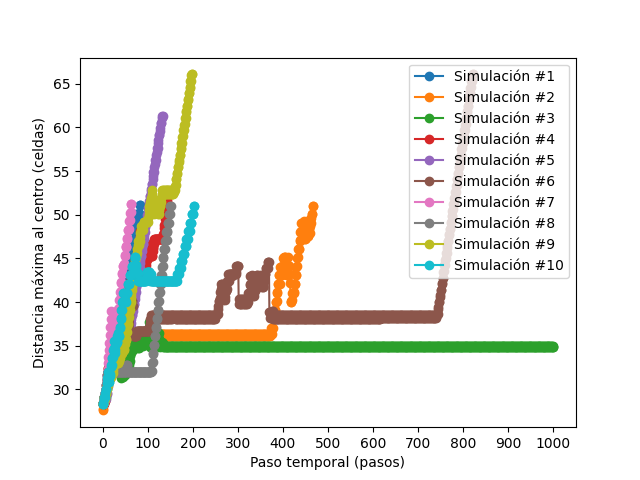
\includegraphics[width=0.8\linewidth]{pic/conway2d/distance_i90}
                \text{$initialLiveCellsProportion = 0.90$}
                \label{fig:conway2d:distance:i90}
            \end{figure}
        }
    \end{multicols}
\end{frame}

\begin{frame}{Conway 2D}
    \textbf{Observable: Tiempo de convergencia al equilibrio}
    \begin{figure}[H]
        \centering
        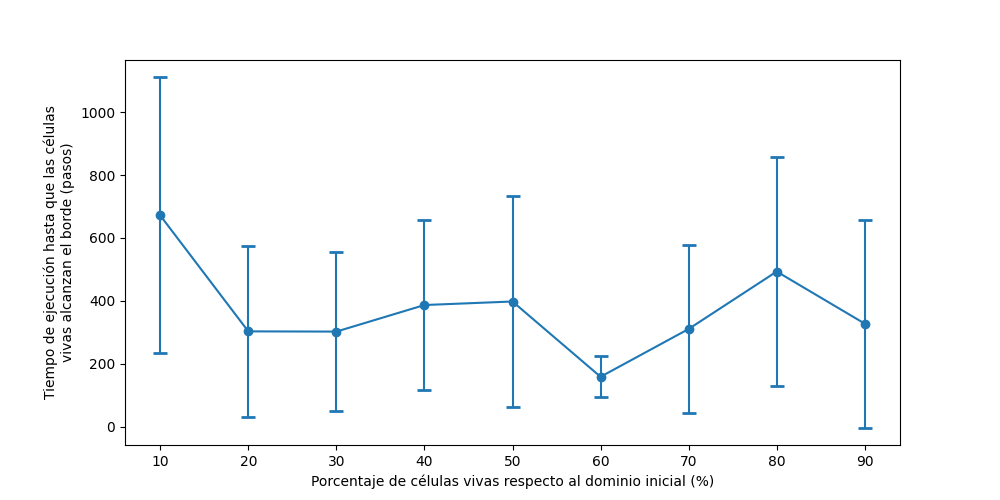
\includegraphics[width=0.8\linewidth]{pic/conway2d/time_vs_input}
        \label{fig:conway2d:time:density}
    \end{figure}
\end{frame}

\begin{frame}{Conway 2D}
    \textbf{Observable: Rapidez de alejamiento de la celda viva más lejana al centro}
    \begin{figure}[H]
        \centering
        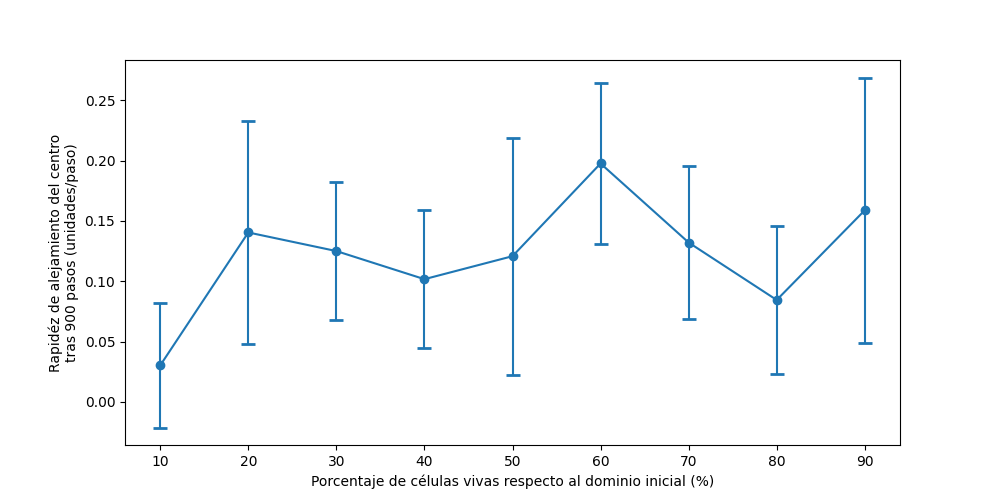
\includegraphics[width=0.8\linewidth]{pic/conway2d/distance_slope_vs_input}
        \label{fig:conway2d:distance_slope:density}
    \end{figure}
\end{frame}


% Sistema 2 Cuarentena 2D

\begin{frame}{Cuarentena 2D}
    \begin{multicols}{2}
        {
            $border = (0, 0) \times (100, 100)$

            $condition = \text{MOORE}$

            $r = 1$

            $shouldKeepAlive = [1, 2, 3, 4, 5, 6, 7, 8]$

            $shouldRevive = [4, 5, 6, 7, 8]$

            $initialDomainProportion = 0.16$

            $initialLiveCellsProportion = 0.50$
        }

        {\begin{figure}[H]
             \centering
             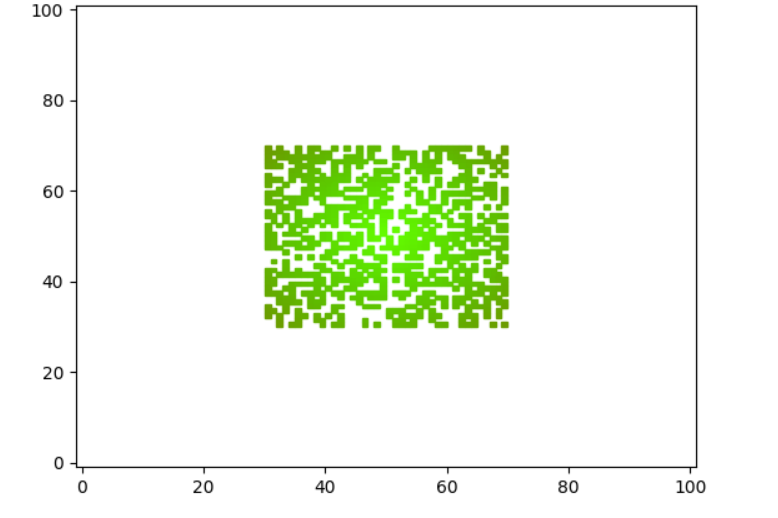
\includegraphics[width=1\linewidth]{pic/cuarentena2d/thumbnail_i50}
             \captionsetup{font={scriptsize}}
             \captionsetup{labelformat=empty}
             \caption{Link al video: https://youtu.be/PfXn3qFnXwE}
             \label{fig:cuarentena2D:thumbnail}
        \end{figure}}
    \end{multicols}
\end{frame}


\begin{frame}{Cuarentena 2D}
    \textcolor{hkustblue}\textbf{Cantidad de celdas vivas en función del tiempo}
    {\footnotesize
    \begin{multicols}{3}
        {
            \begin{figure}[H]
                \centering
                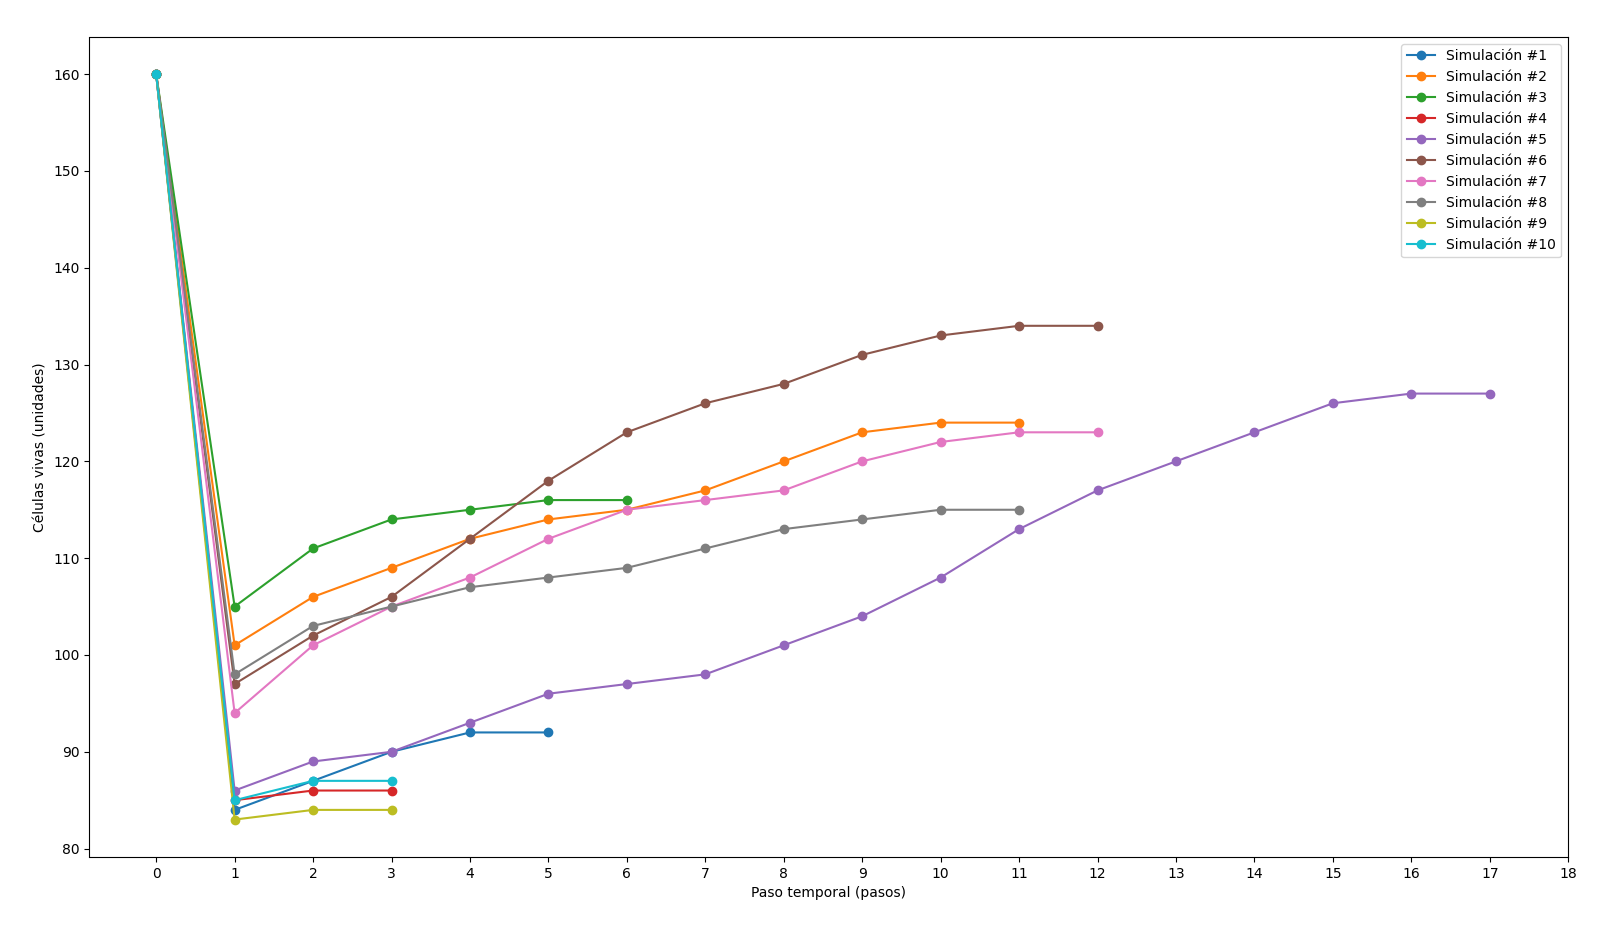
\includegraphics[width=0.8\linewidth]{pic/cuarentena2d/size_i10}
                \text{$initialLiveCellsProportion = 0.10$}
                \label{fig:cuarentena:size:i10}
            \end{figure}
        }

        {
            \begin{figure}[H]
                \centering
                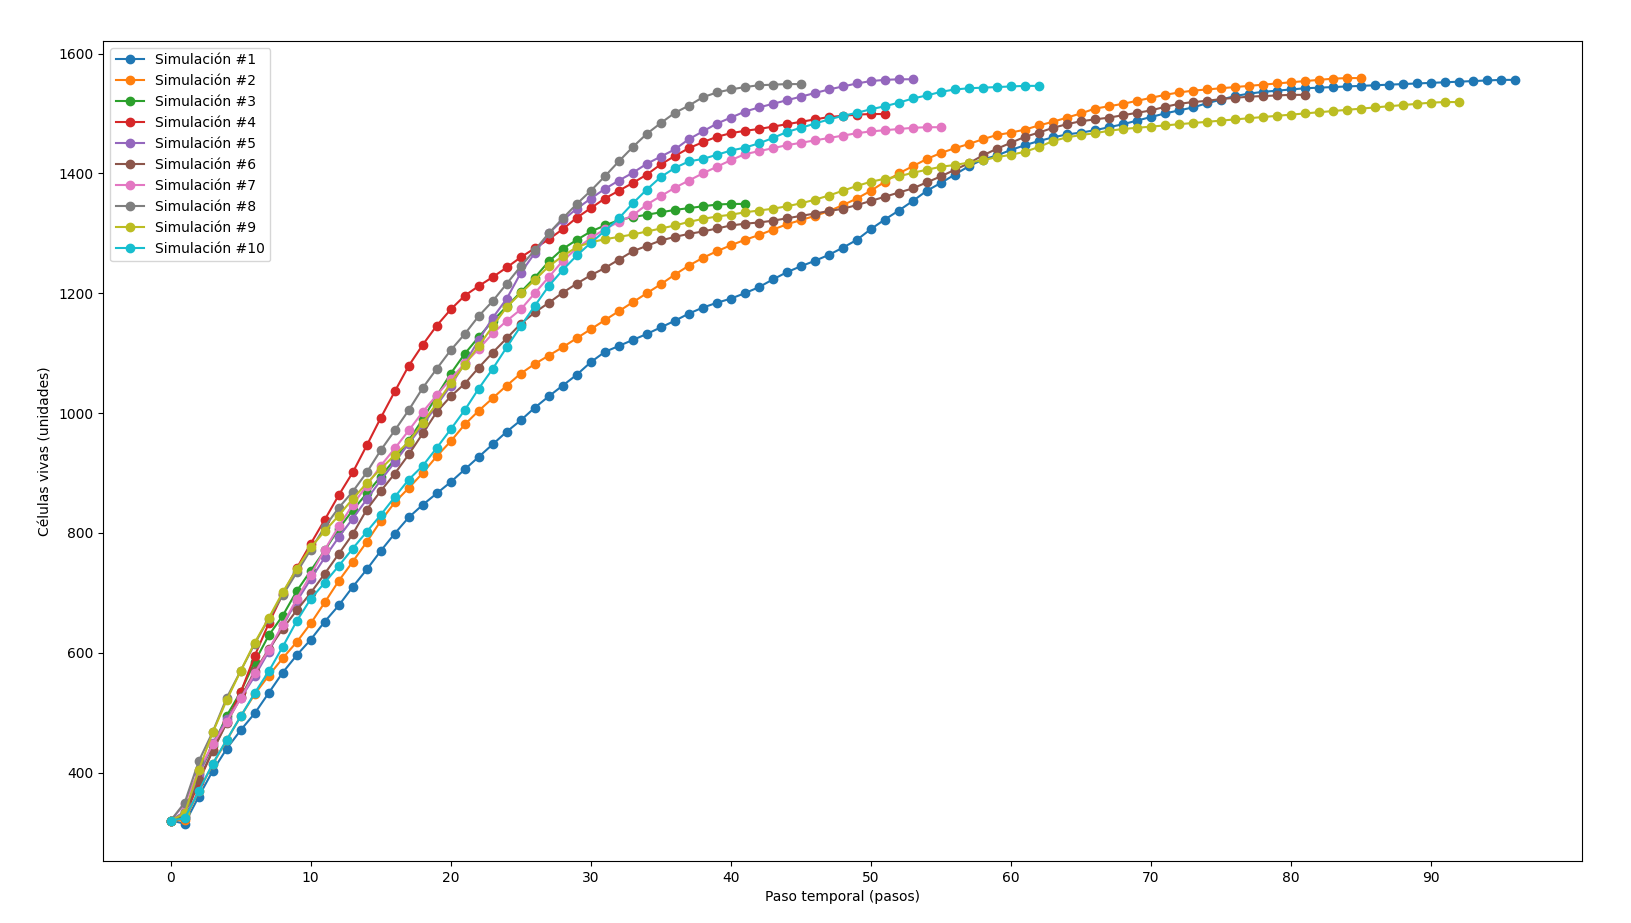
\includegraphics[width=0.8\linewidth]{pic/cuarentena2d/size_i20}
                \text{$initialLiveCellsProportion = 0.20$}
                \label{fig:cuarentena:size:i20}
            \end{figure}
        }

        {
            \begin{figure}[H]
                \centering
                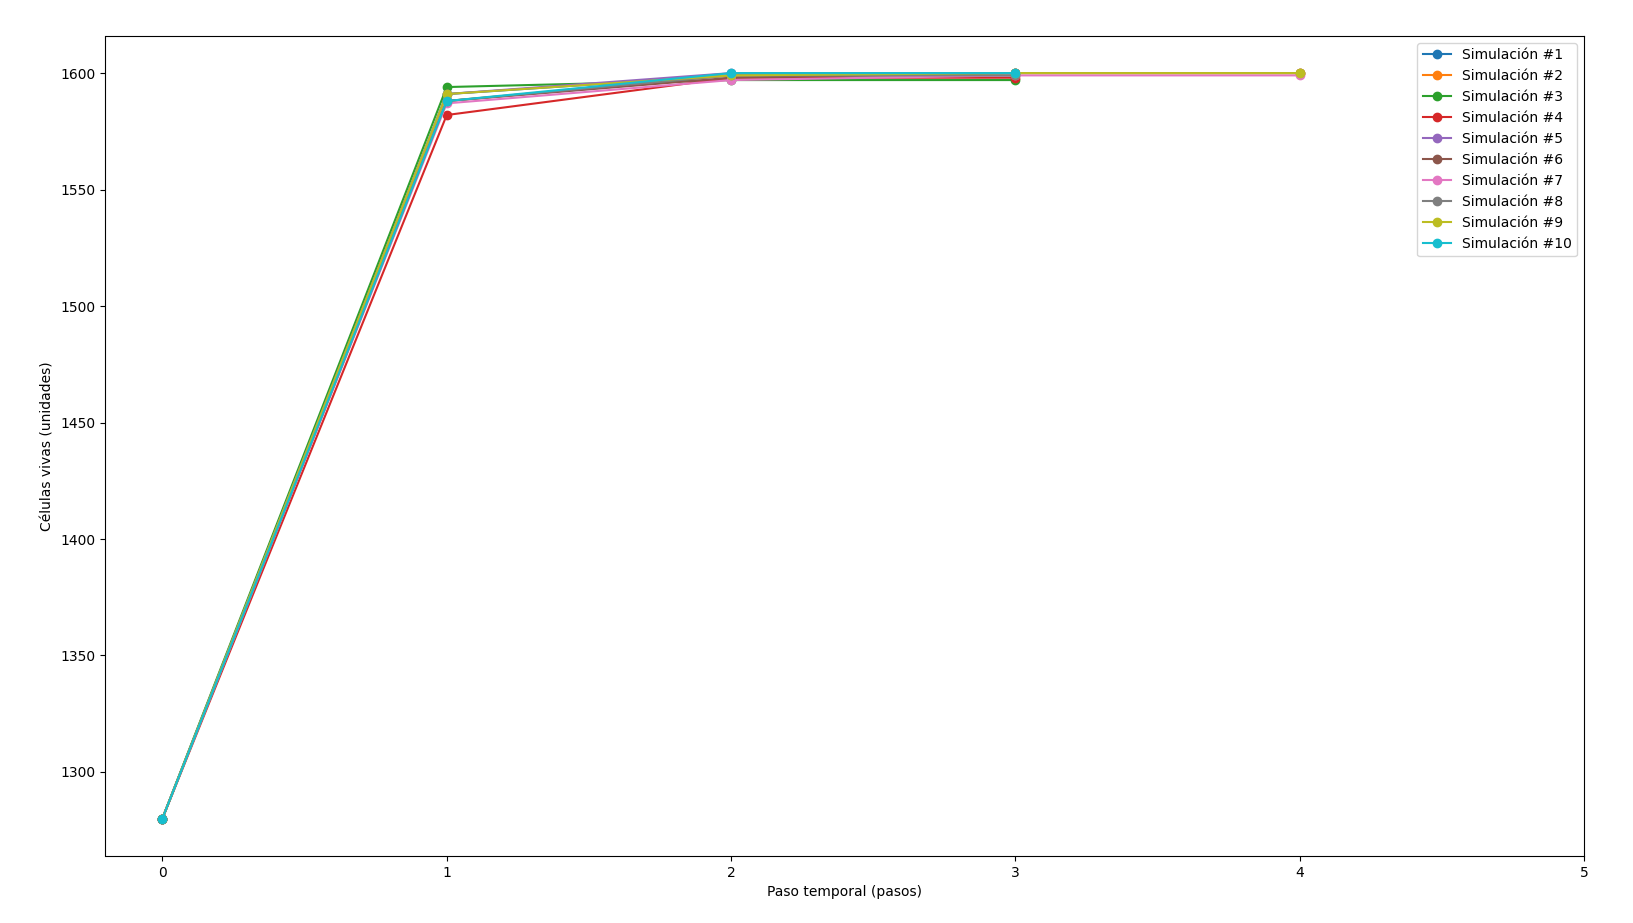
\includegraphics[width=0.8\linewidth]{pic/cuarentena2d/size_i80}
                \text{$initialLiveCellsProportion = 0.80$}
                \label{fig:cuarentena:size:i80}
            \end{figure}
        }
    \end{multicols}
    }
\end{frame}


\begin{frame}{Cuarentena 2D}
    \textbf{Observable: Variación cantidad de celdas vivas}
    \begin{figure}[H]
        \centering
        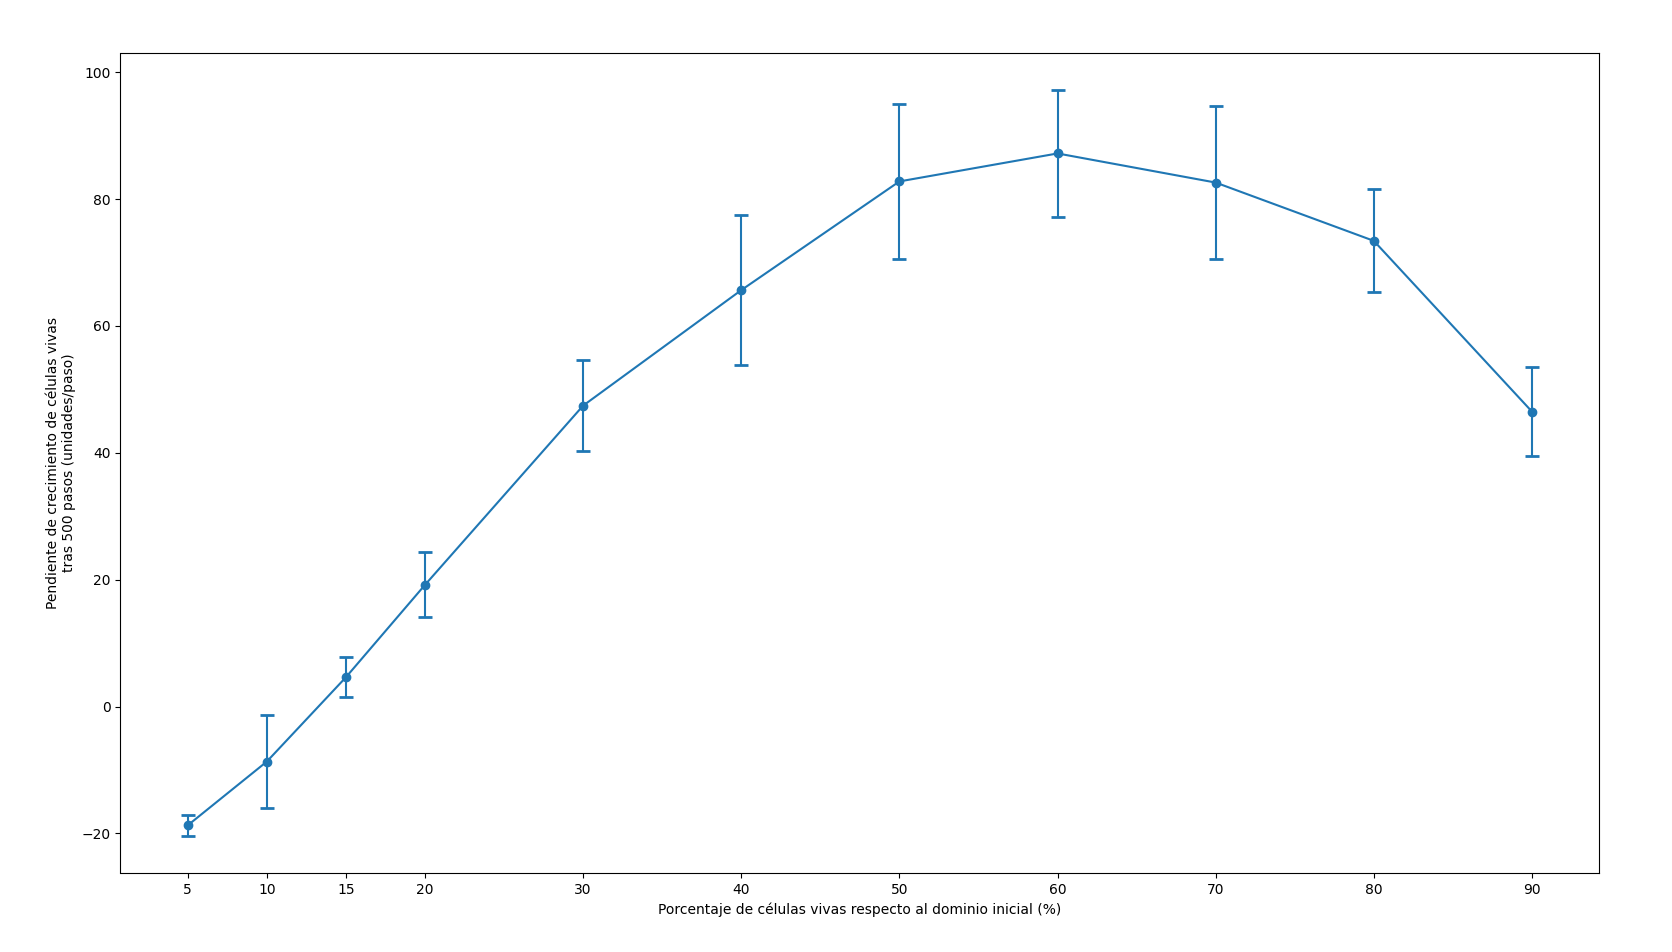
\includegraphics[width=0.8\linewidth]{pic/cuarentena2d/observable}
        \label{fig:cuarentena:size:slope}
    \end{figure}
\end{frame}



% Sistema 3 Expansión circular 2D

\begin{frame}{Expansión circular 2D}
    \begin{multicols}{2}
        {
            $border = (0, 0) \times (100, 100)$

            $condition = \text{MOORE}$

            $r = 1$

            $shouldKeepAlive = [0, 1, 4, 5, 6, 7, 8]$

            $shouldRevive = [2, 3]$

            $initialDomainProportion = 0.16$

            $initialLiveCellsProportion = 0.60$
        }

        {\begin{figure}[H]
             \centering
             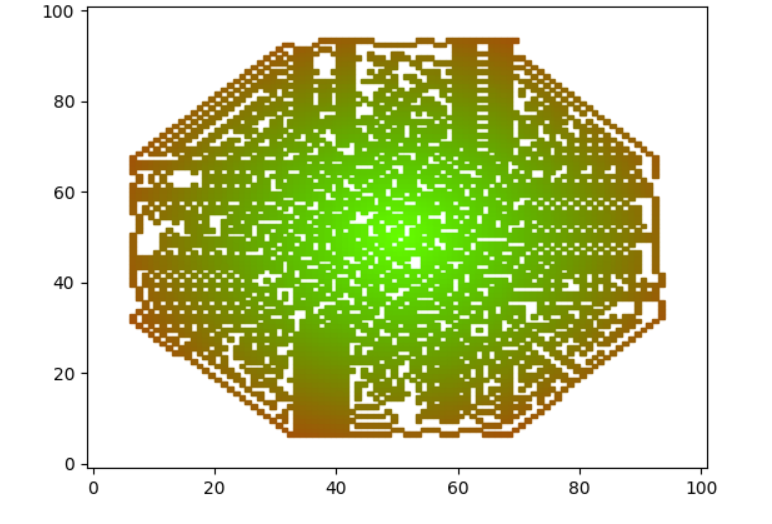
\includegraphics[width=1\linewidth]{pic/circular2d/thumbnail}
             \captionsetup{font={scriptsize}}
             \captionsetup{labelformat=empty}
             \caption{Link al video: https://youtu.be/BShT8UAhHek}
             \label{fig:expcirc2d:thumbnail}
        \end{figure}}
    \end{multicols}
\end{frame}


\begin{frame}{Expansión circular 2D}
    \textbf{Cantidad de celdas vivas en función del tiempo}
    \begin{multicols}{2}
        {
            \begin{figure}[H]
                \centering
                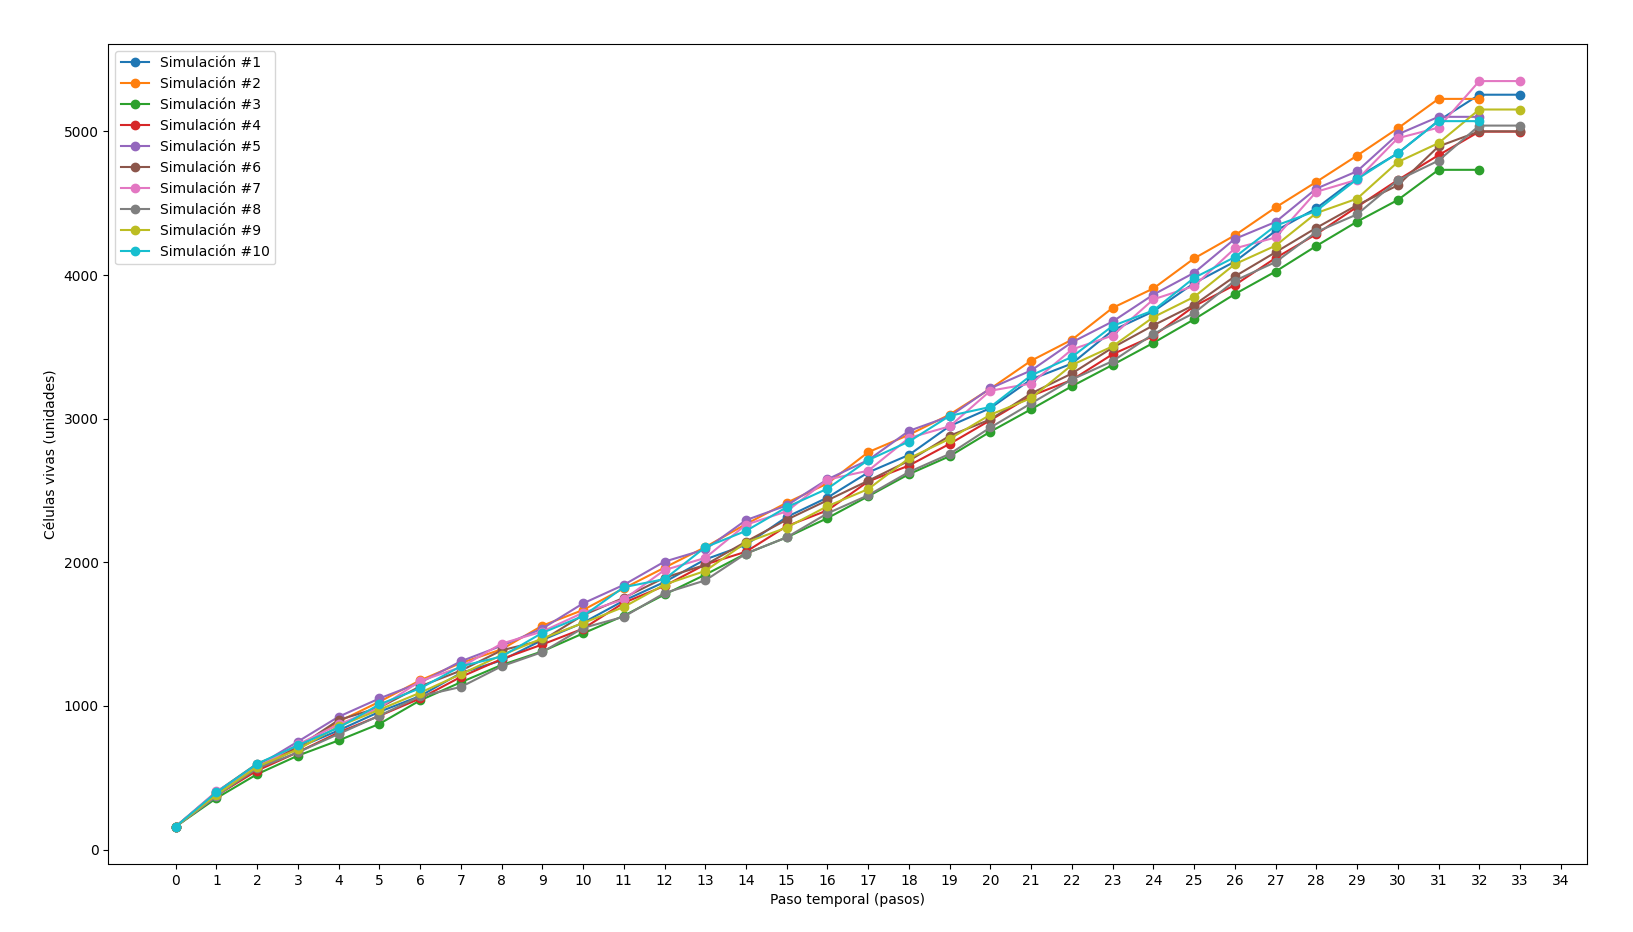
\includegraphics[width=0.8\linewidth]{pic/circular2d/size_i10}
                \text{$initialLiveCellsProportion = 0.10$}
                \label{fig:expcirc:size:i10}
            \end{figure}
        }

        {
            \begin{figure}[H]
                \centering
                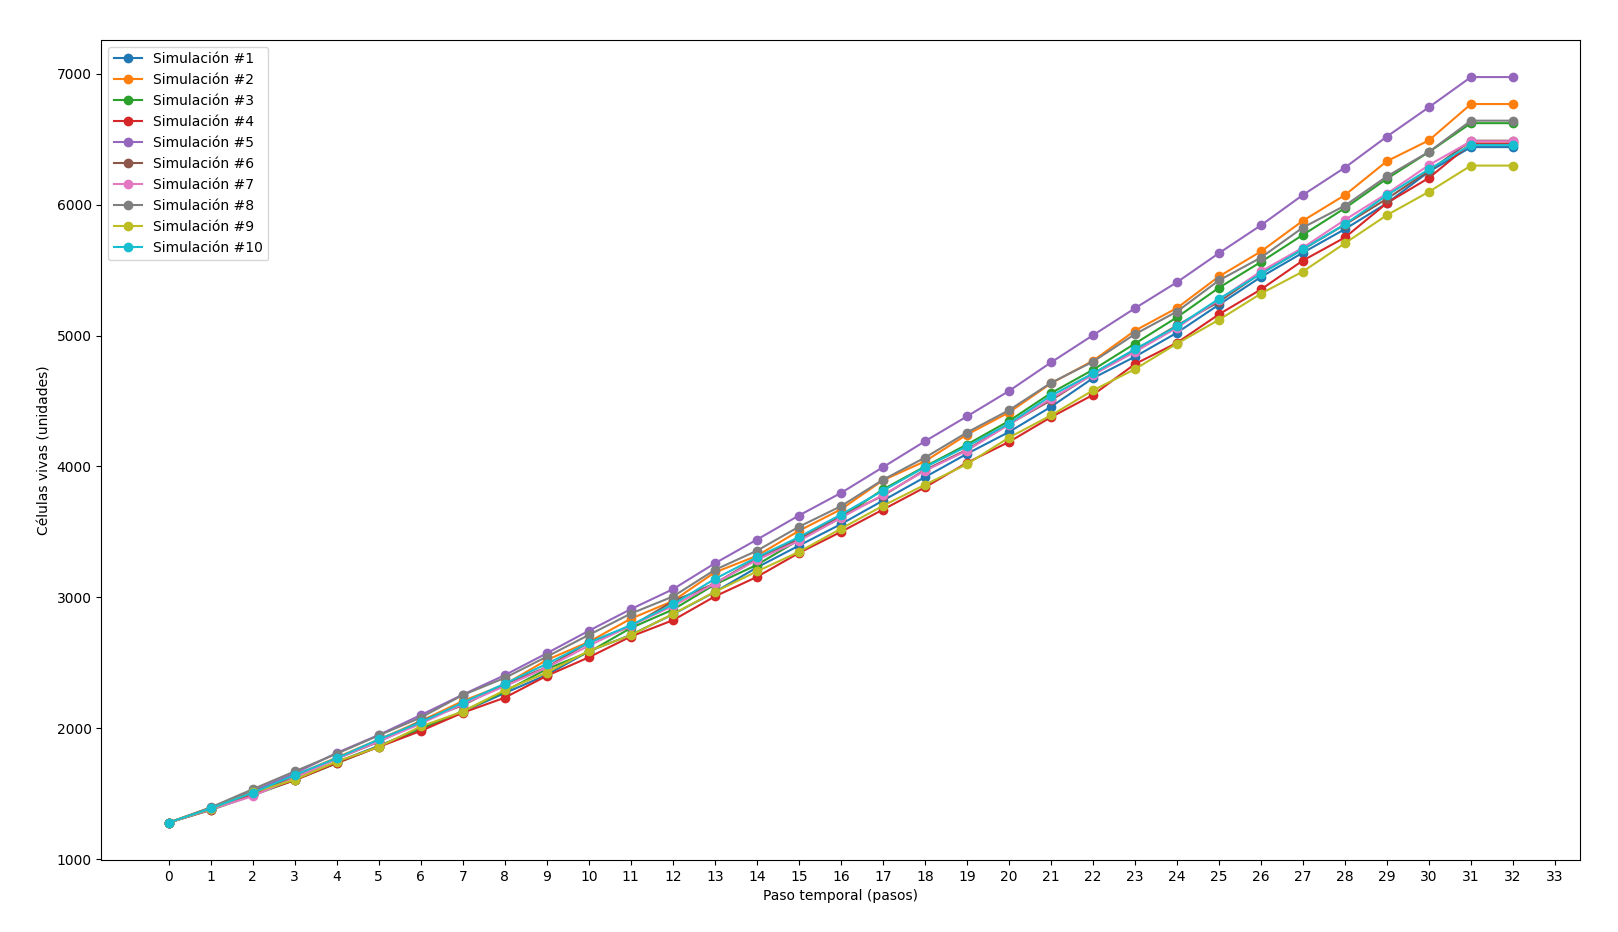
\includegraphics[width=0.8\linewidth]{pic/circular2d/size_i80}
                \text{$initialLiveCellsProportion = 0.80$}
                \label{fig:expcirc:size:i80}
            \end{figure}
        }
    \end{multicols}
\end{frame}


\begin{frame}{Expansión circular 2D}
    \textbf{Observable: Cantidad de celdas vivas}
    \begin{figure}[H]
        \centering
        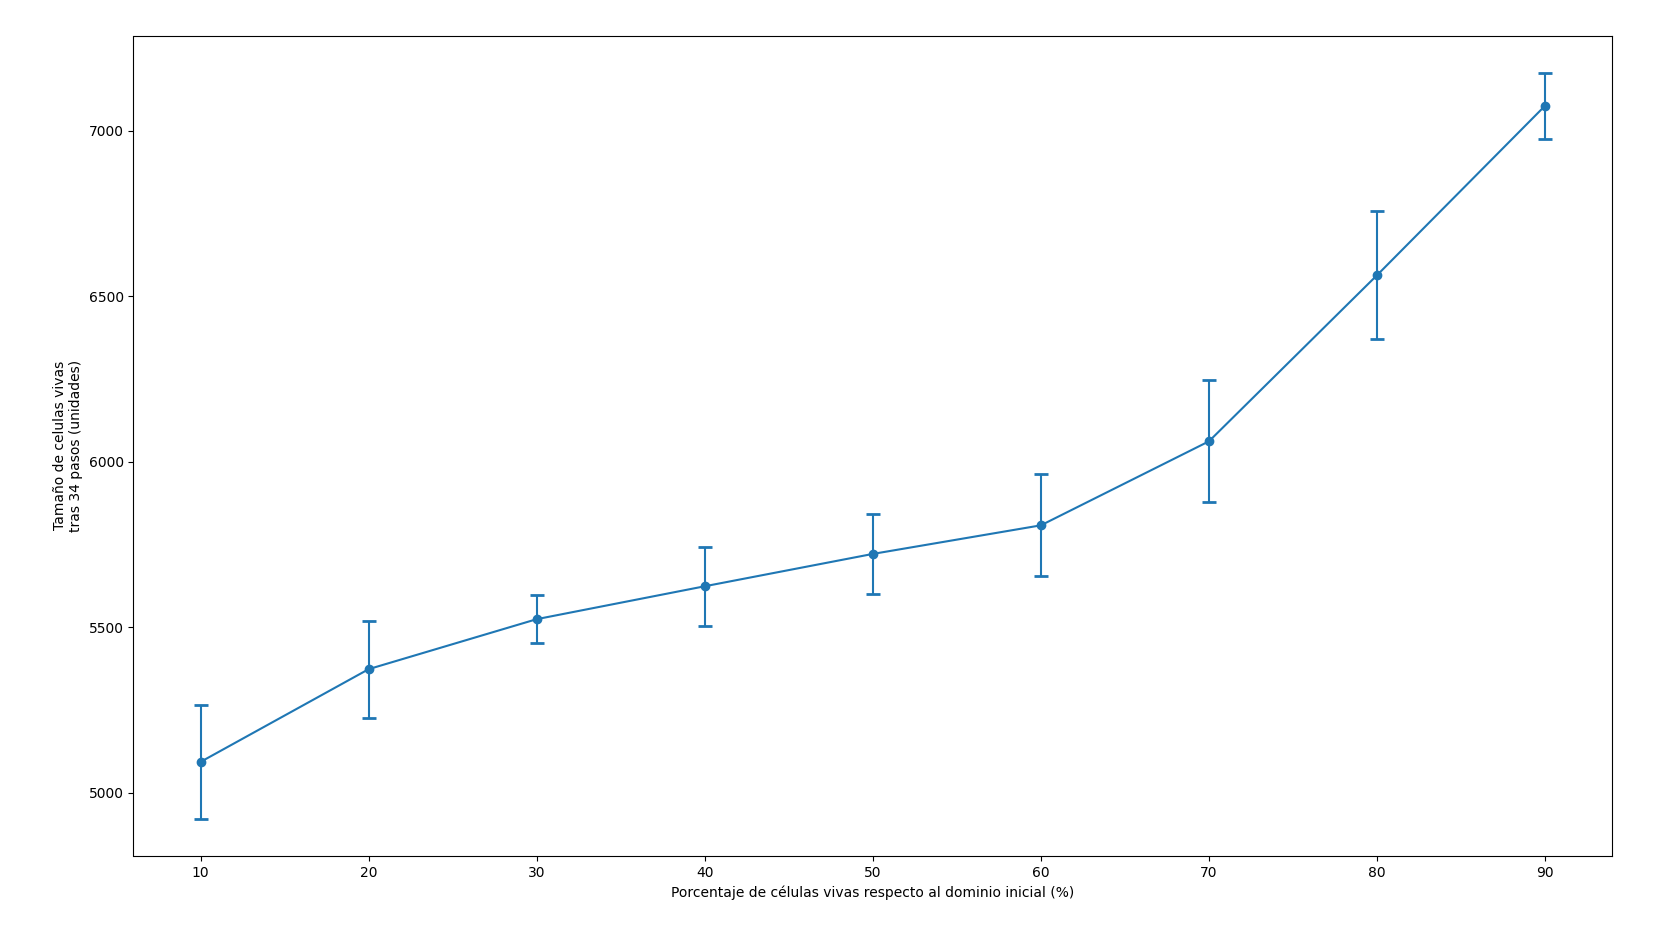
\includegraphics[width=0.8\linewidth]{pic/circular2d/observable}
        \label{fig:expcirc:size}
    \end{figure}
\end{frame}





% Sistema 4 Conway 3D

\begin{frame}{Conway 3D}
    \begin{multicols}{2}
        {
            $border = (0, 0, 0) \times (50, 50, 50)$

            $condition = \text{MOORE}$

            $r = 1$

            $shouldKeepAlive = [2, 3]$

            $shouldRevive = [3]$

            $initialDomainProportion = 0.064$

            $initialLiveCellsProportion = 0.50$
        }

        {\begin{figure}[H]
             \centering
             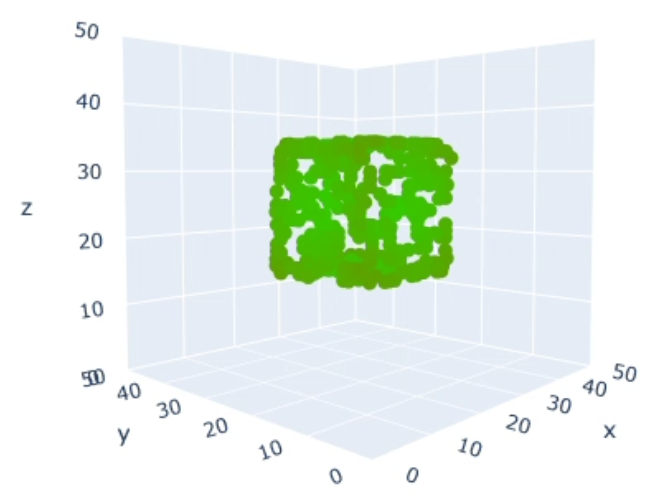
\includegraphics[width=1\linewidth]{pic/conway3d/thumbnail_i50}
             \captionsetup{font={scriptsize}}
             \captionsetup{labelformat=empty}
             \caption{Link al video: https://youtu.be/HlUXy0G1ep0}
             \label{fig:conway3D:thumbnail}
        \end{figure}}
    \end{multicols}
\end{frame}


\begin{frame}{Conway 3D}
    \textbf{Cantidad de celdas vivas en función del tiempo}
    \begin{multicols}{2}
        {
            \begin{figure}[H]
                \centering
                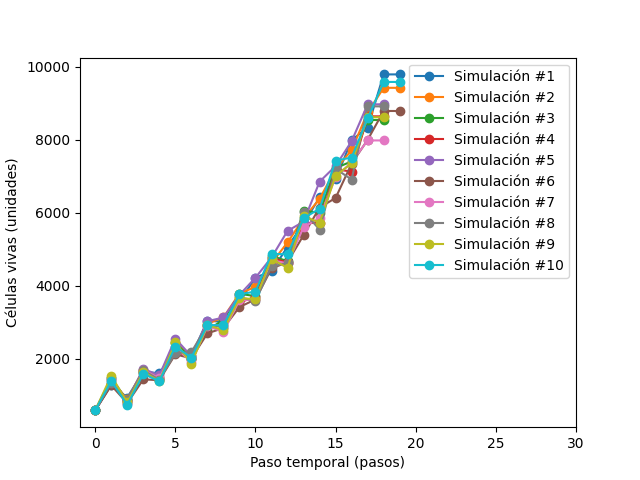
\includegraphics[width=0.8\linewidth]{pic/conway3d/size_i10}
                \text{$initialLiveCellsProportion = 0.10$}
                \label{fig:conway3d:size:i10}
            \end{figure}
        }

        {
            \begin{figure}[H]
                \centering
                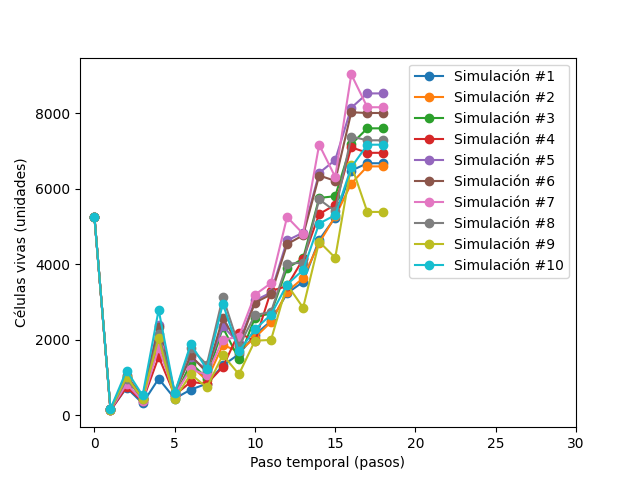
\includegraphics[width=0.8\linewidth]{pic/conway3d/size_i90}
                \text{$initialLiveCellsProportion = 0.90$}
                \label{fig:conway3d:size:i90}
            \end{figure}
        }
    \end{multicols}
\end{frame}

\begin{frame}{Conway 3D}
    \textbf{Observable: Cantidad de celdas vivas en el equilibrio}
    \begin{figure}[H]
        \centering
        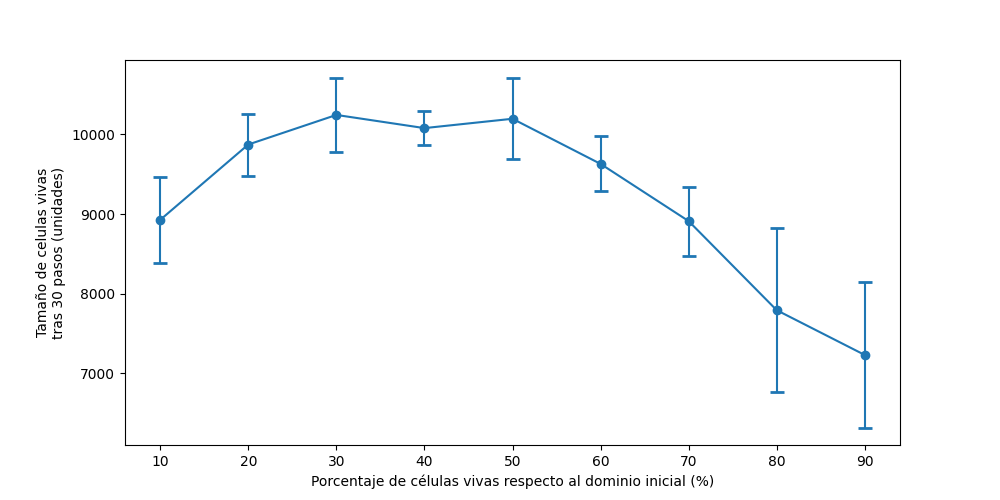
\includegraphics[width=0.8\linewidth]{pic/conway3d/size_vs_input}
        \label{fig:conway3d:size:density}
    \end{figure}
\end{frame}

\begin{frame}{Conway 3D}
    \textbf{Observable: Variación de la cantidad de celdas vivas}
    \begin{figure}[H]
        \centering
        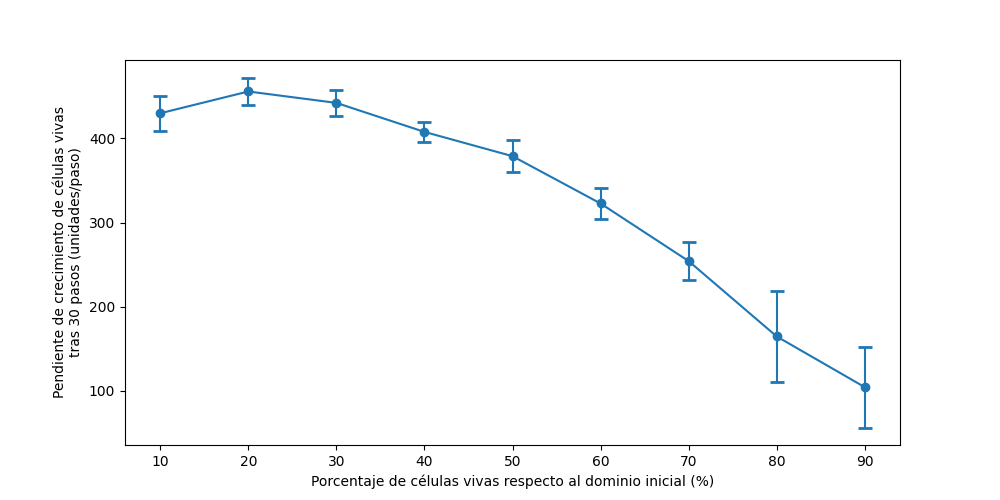
\includegraphics[width=0.8\linewidth]{pic/conway3d/size_slope_vs_input}
        \label{fig:conway3d:size_slope:density}
    \end{figure}
\end{frame}

\begin{frame}{Conway 3D}
    \textbf{Distancia de la celda viva más lejana al centro en función del tiempo}
    \begin{multicols}{2}
        {
            \begin{figure}[H]
                \centering
                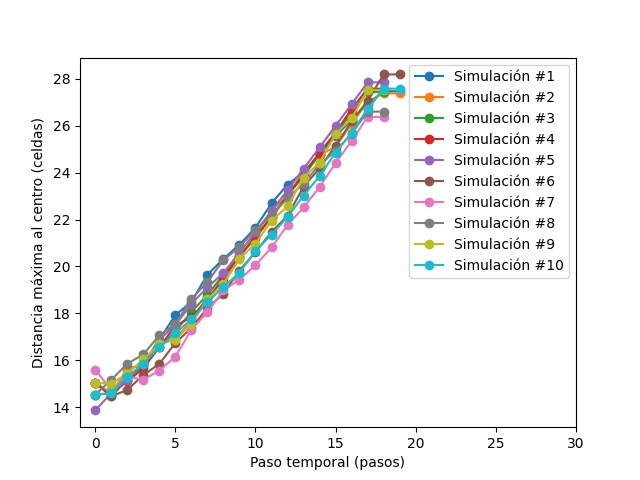
\includegraphics[width=0.8\linewidth]{pic/conway3d/distance_i10}
                \text{$initialLiveCellsProportion = 0.10$}
                \label{fig:conway3d:distance:i10}
            \end{figure}
        }

        {
            \begin{figure}[H]
                \centering
                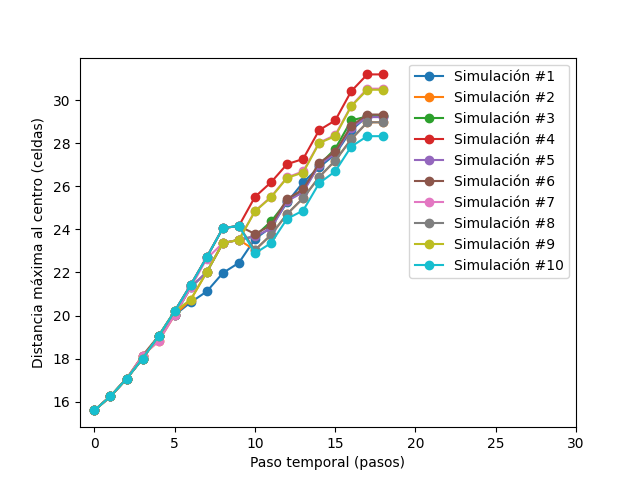
\includegraphics[width=0.8\linewidth]{pic/conway3d/distance_i90}
                \text{$initialLiveCellsProportion = 0.90$}
                \label{fig:conway3d:distance:i90}
            \end{figure}
        }
    \end{multicols}
\end{frame}

\begin{frame}{Conway 3D}
    \textbf{Observable: Tiempo de convergencia al equilibrio}
    \begin{figure}[H]
        \centering
        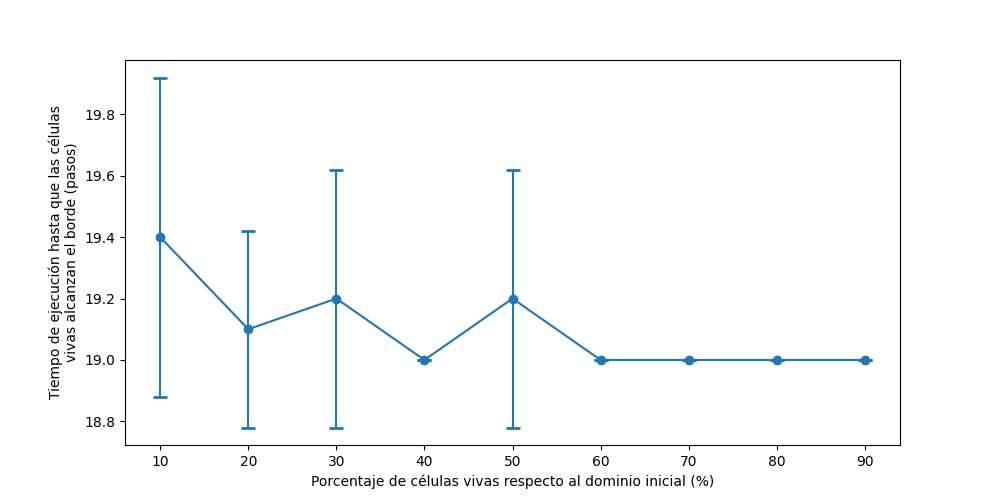
\includegraphics[width=0.8\linewidth]{pic/conway3d/time_vs_input}
        \label{fig:conway3d:time:density}
    \end{figure}
\end{frame}

\begin{frame}{Conway 3D}
    \textbf{Observable: Rapidez de alejamiento de la celda viva más lejana al centro}
    \begin{figure}[H]
        \centering
        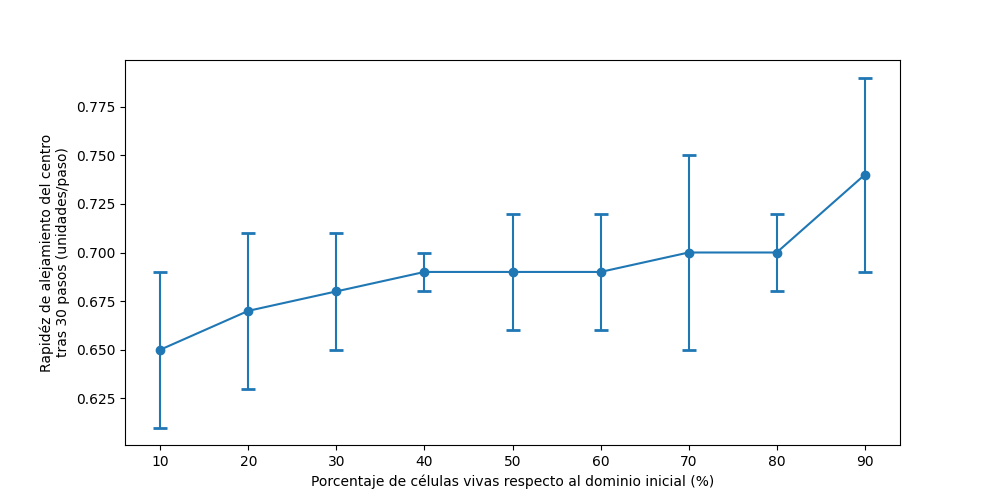
\includegraphics[width=0.8\linewidth]{pic/conway3d/distance_slope_vs_input}
        \label{fig:conway3d:distance_slope:density}
    \end{figure}
\end{frame}



% Sistema 5 Colapso Cubico

\begin{frame}{Colapso cúbico}
    \begin{multicols}{2}
        {
            $border = (0, 0, 0) \times (50, 50, 50)$

            $condition = \text{VON}\_\text{NEUMANN}$

            $r = 1$

            $shouldKeepAlive = [0]$

            $shouldRevive = [2]$

            $initialDomainProportion = 0.064$

            $initialLiveCellsProportion = 0.30$
        }

        {\begin{figure}[H]
             \centering
             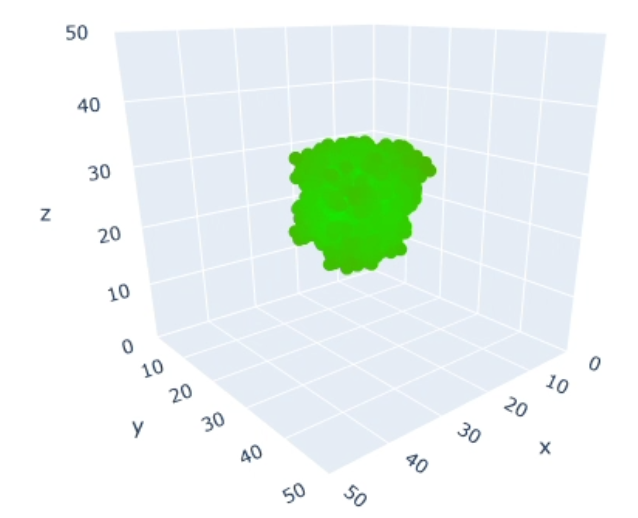
\includegraphics[width=1\linewidth]{pic/collapse3d/thumbnail_i30}
             \captionsetup{font={scriptsize}}
             \captionsetup{labelformat=empty}
             \caption{Link al video: https://youtu.be/UeXUv7qMRoU}
             \label{fig:colapso3d:thumbnail}
        \end{figure}}
    \end{multicols}
\end{frame}


\begin{frame}{Colapso cúbico}
    \textbf{Cantidad de celdas vivas en función del tiempo}
    {\footnotesize
    \begin{multicols}{3}
        {
            \begin{figure}[H]
                \centering
                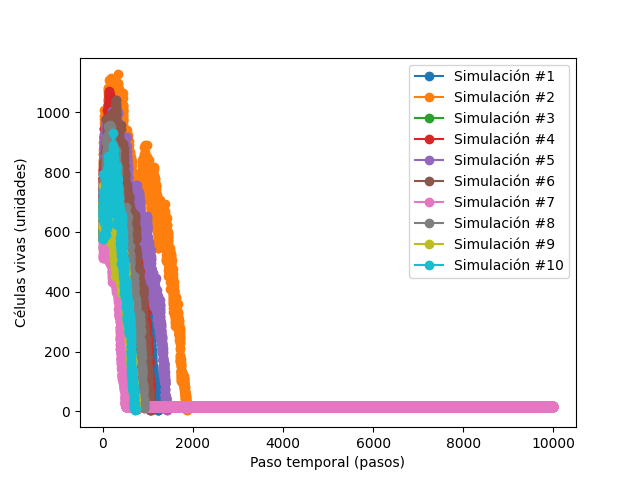
\includegraphics[width=0.8\linewidth]{pic/collapse3d/size_i10}
                \text{$initialLiveCellsProportion = 0.10$}
                \label{fig:colapso:size:i10}
            \end{figure}
        }

        {
            \begin{figure}[H]
                \centering
                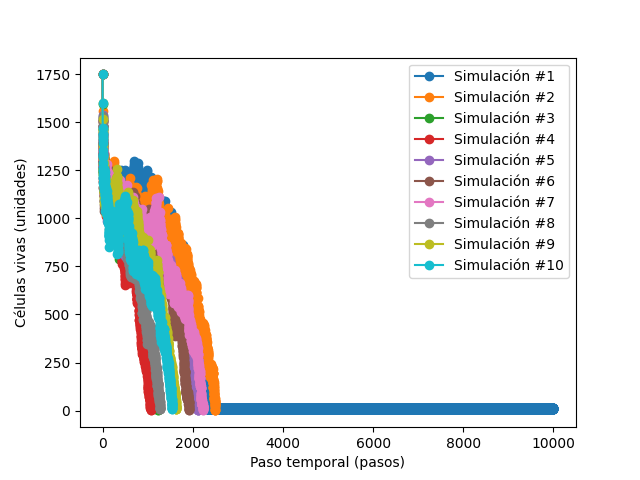
\includegraphics[width=0.8\linewidth]{pic/collapse3d/size_i30}
                \text{$initialLiveCellsProportion = 0.30$}
                \label{fig:colapso:size:i30}
            \end{figure}
        }

        {
            \begin{figure}[H]
                \centering
                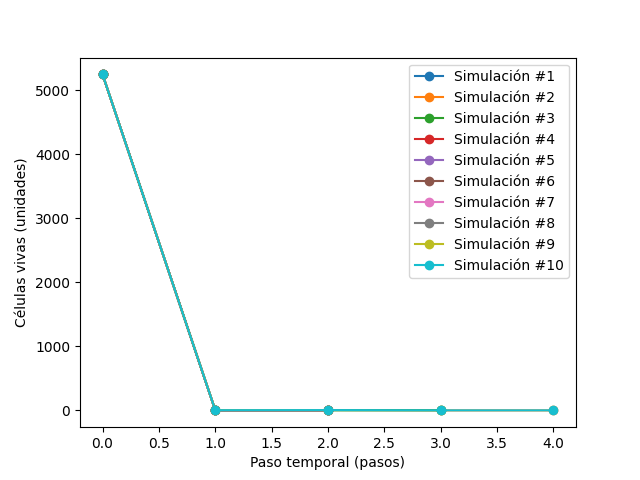
\includegraphics[width=0.8\linewidth]{pic/collapse3d/size_i90}
                \text{$initialLiveCellsProportion = 0.90$}
                \label{fig:colapso:size:i90}
            \end{figure}
        }
    \end{multicols}
    }
\end{frame}

\begin{frame}{Colapso cúbico}
    \textbf{Observable: Cantidad de celdas vivas en el equilibrio}
    \begin{figure}[H]
        \centering
        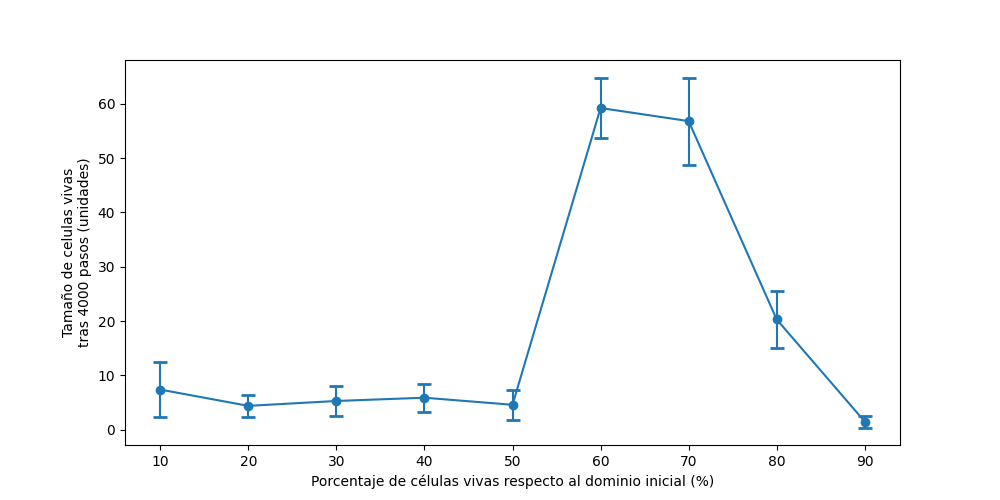
\includegraphics[width=0.8\linewidth]{pic/collapse3d/size_vs_input}
        \label{fig:colapso:size:density}
    \end{figure}
\end{frame}

\begin{frame}{Colapso cúbico}
    \textbf{Observable: Variación de cantidad de celdas vivas}
    \begin{figure}[H]
        \centering
        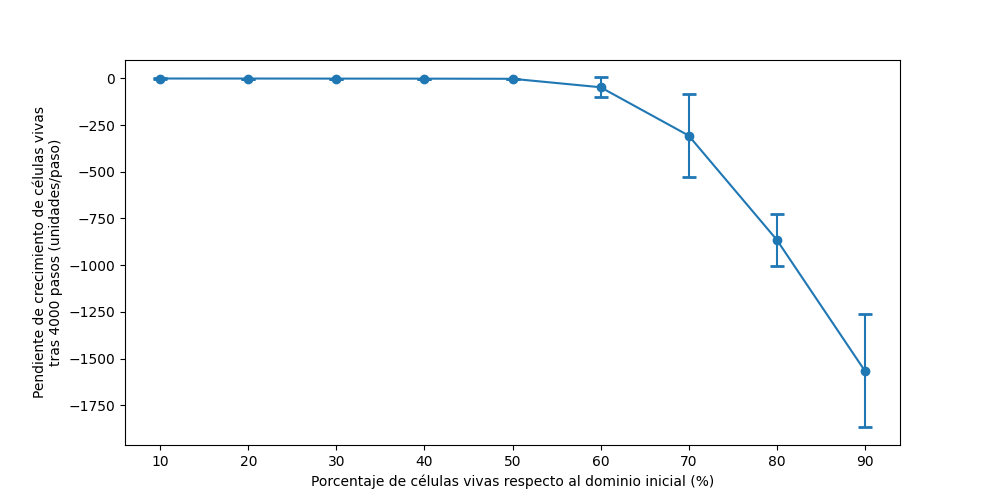
\includegraphics[width=0.8\linewidth]{pic/collapse3d/size_slope_vs_input}
        \label{fig:colapso:size_slope:density}
    \end{figure}
\end{frame}


\begin{frame}{Colapso cúbico}
    \textbf{Distancia de la celda viva más lejana al centro en función del tiempo}
    {\footnotesize
    \begin{multicols}{3}
        {
            \begin{figure}[H]
                \centering
                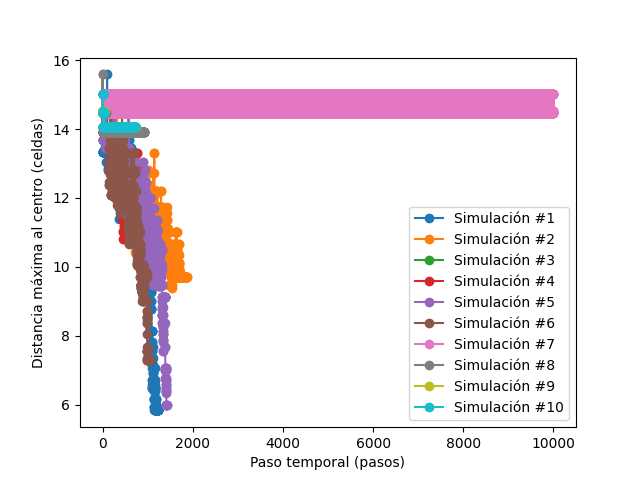
\includegraphics[width=0.8\linewidth]{pic/collapse3d/distance_i10}
                \text{$initialLiveCellsProportion = 0.10$}
                \label{fig:colapso:distance:i10}
            \end{figure}
        }

        {
            \begin{figure}[H]
                \centering
                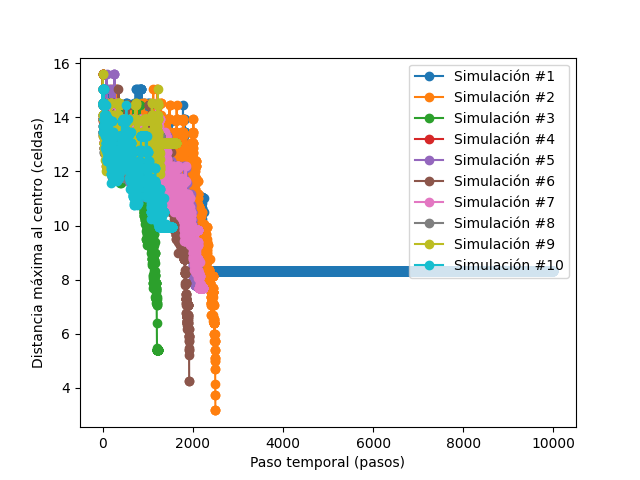
\includegraphics[width=0.8\linewidth]{pic/collapse3d/distance_i30}
                \text{$initialLiveCellsProportion = 0.30$}
                \label{fig:colapso:distance:i30}
            \end{figure}
        }

        {
            \begin{figure}[H]
                \centering
                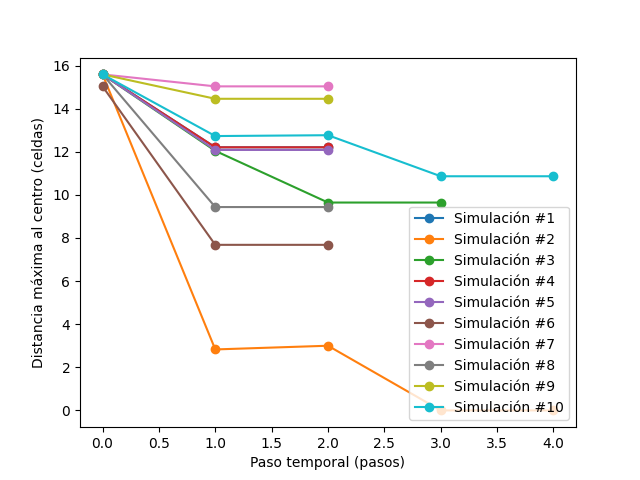
\includegraphics[width=0.8\linewidth]{pic/collapse3d/distance_i90}
                \text{$initialLiveCellsProportion = 0.90$}
                \label{fig:colapso:distance:i90}
            \end{figure}
        }
    \end{multicols}
    }
\end{frame}

\begin{frame}{Colapso cúbico}
    \textbf{Observable: Rapidez de alejamiento de la celda viva más lejana al centro}
    \begin{figure}[H]
        \centering
        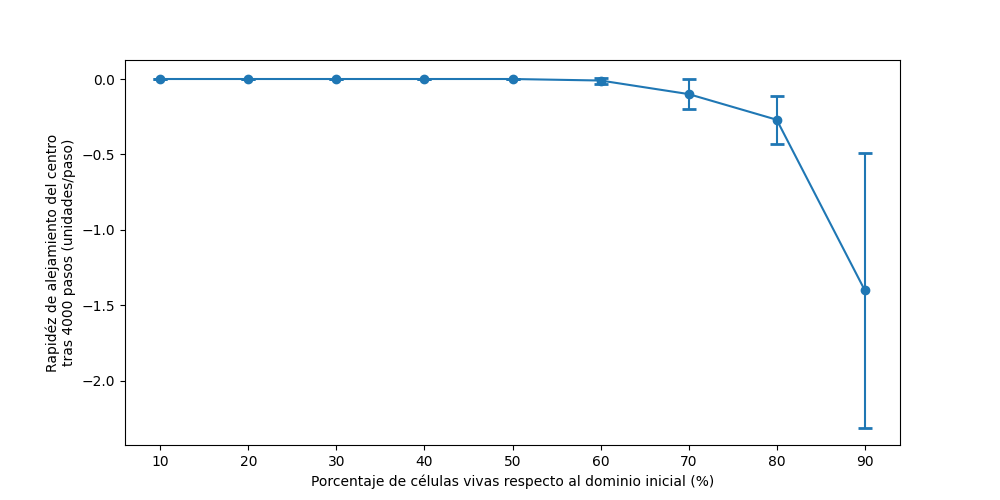
\includegraphics[width=0.8\linewidth]{pic/collapse3d/distance_slope_vs_input}
        \label{fig:colapso:distance_slope:density}
    \end{figure}
\end{frame}



% Sistema 6 Expansión cúbica 3D

\begin{frame}{Expansión cúbica 3D}
    \begin{multicols}{2}
        {
            $border = (0, 0, 0) \times (50, 50, 50)$

            $condition = \text{MOORE}$

            $r = 1$

            $shouldKeepAlive = [0, 1, 2, 3, 4, 5, 6, 7, 8]$

            $shouldRevive = [1, 2, 3]$

            $initialDomainProportion = 0.064$

            $initialLiveCellsProportion = 0.90$
        }

        {\begin{figure}[H]
             \centering
             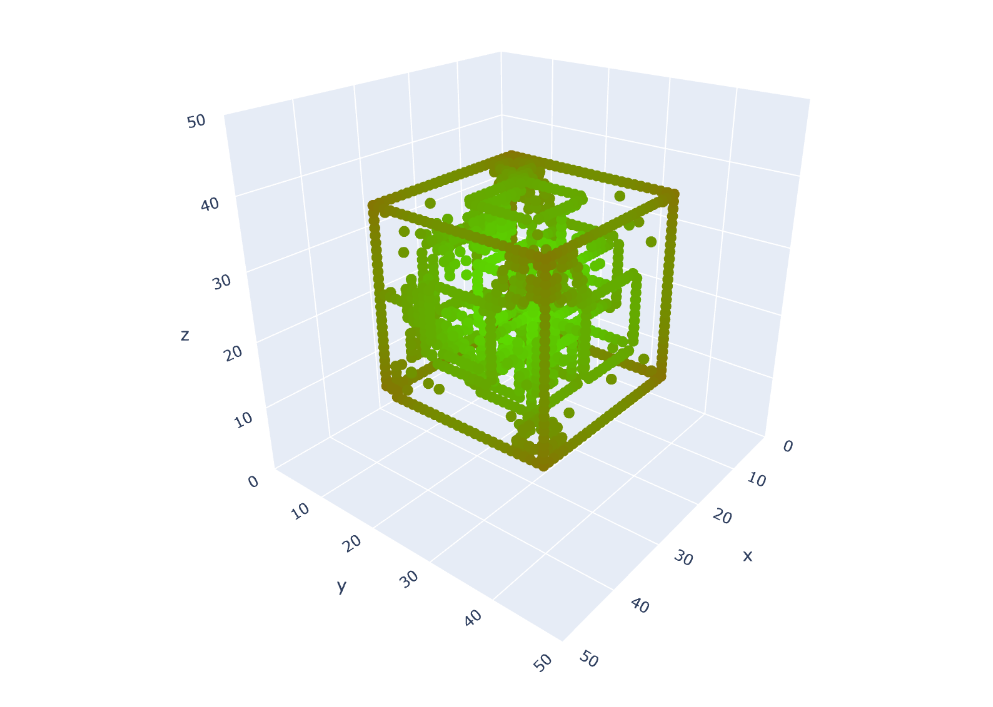
\includegraphics[width=1\linewidth]{pic/cubo3d/thumbnail}
             \captionsetup{font={scriptsize}}
             \captionsetup{labelformat=empty}
             \caption{Link al video: https://youtu.be/Zu9bqnto0ak}
             \label{fig:expcub3d:thumbnail}
        \end{figure}}
    \end{multicols}
\end{frame}



\begin{frame}{Expansión cúbica 3D}
    \textbf{Cantidad de celdas vivas en función del tiempo}
    \begin{multicols}{2}
        {
            \begin{figure}[H]
                \centering
                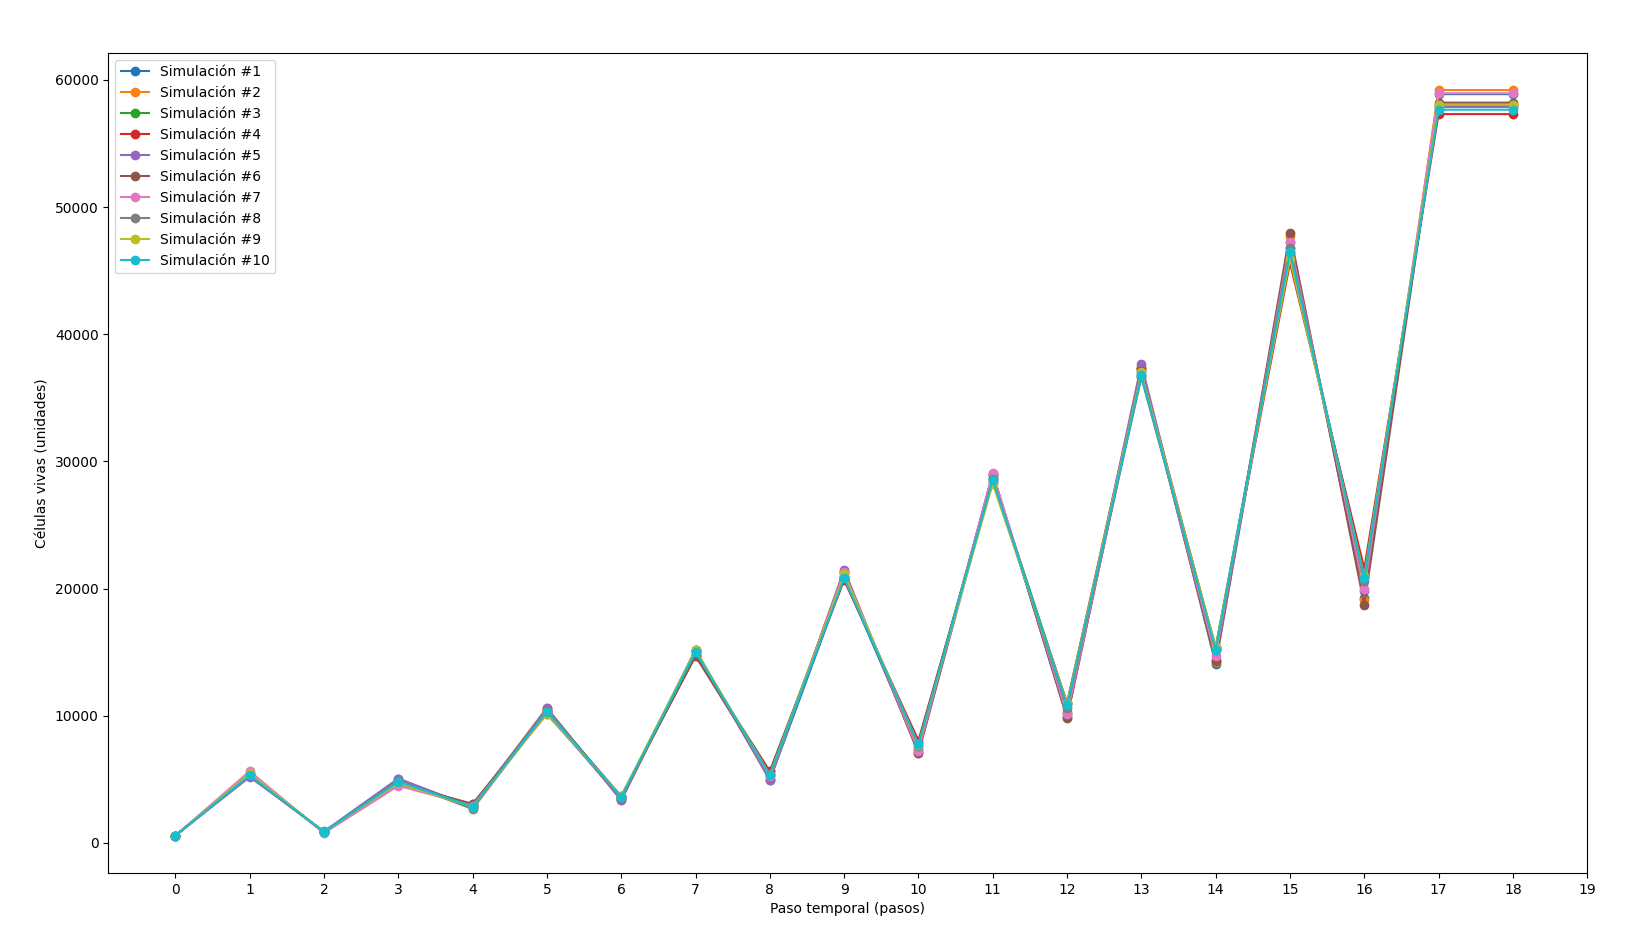
\includegraphics[width=0.8\linewidth]{pic/cubo3d/size_i10}
                \text{$initialLiveCellsProportion = 0.10$}
                \label{fig:expcub:size:i10}
            \end{figure}
        }

        {
            \begin{figure}[H]
                \centering
                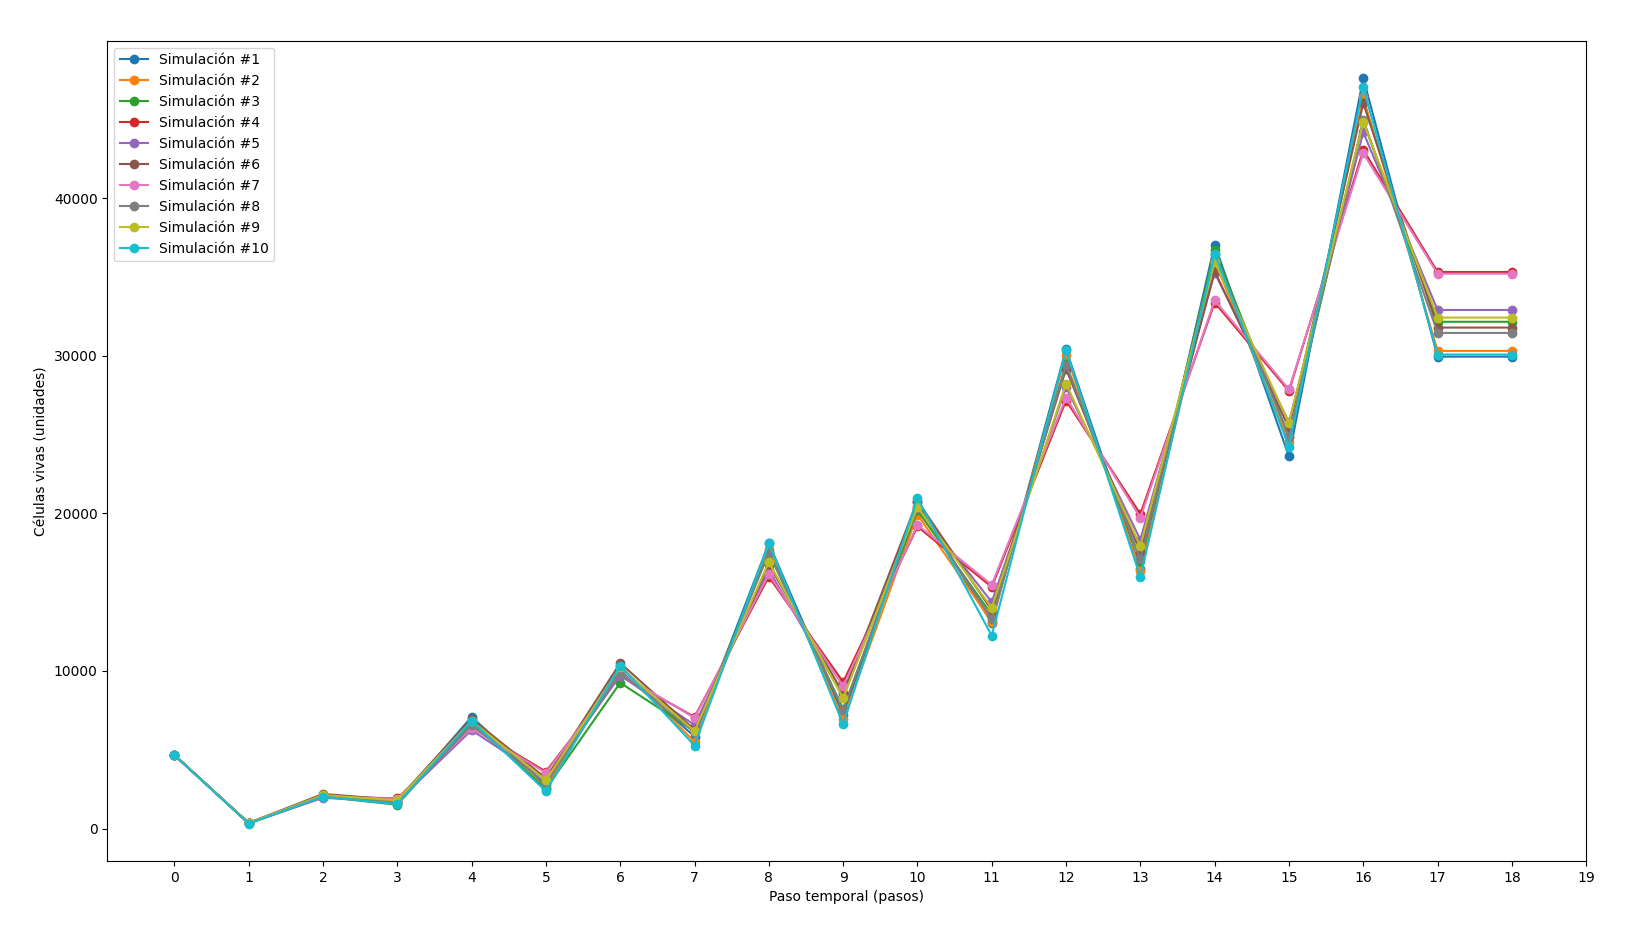
\includegraphics[width=0.8\linewidth]{pic/cubo3d/size_i80}
                \text{$initialLiveCellsProportion = 0.80$}
                \label{fig:expcub:size:i80}
            \end{figure}
        }
    \end{multicols}
\end{frame}


\begin{frame}{Expansión cúbica 3D}
    \textbf{Observable: Variación de la cantidad de celdas vivas}
    \begin{figure}[H]
        \centering
        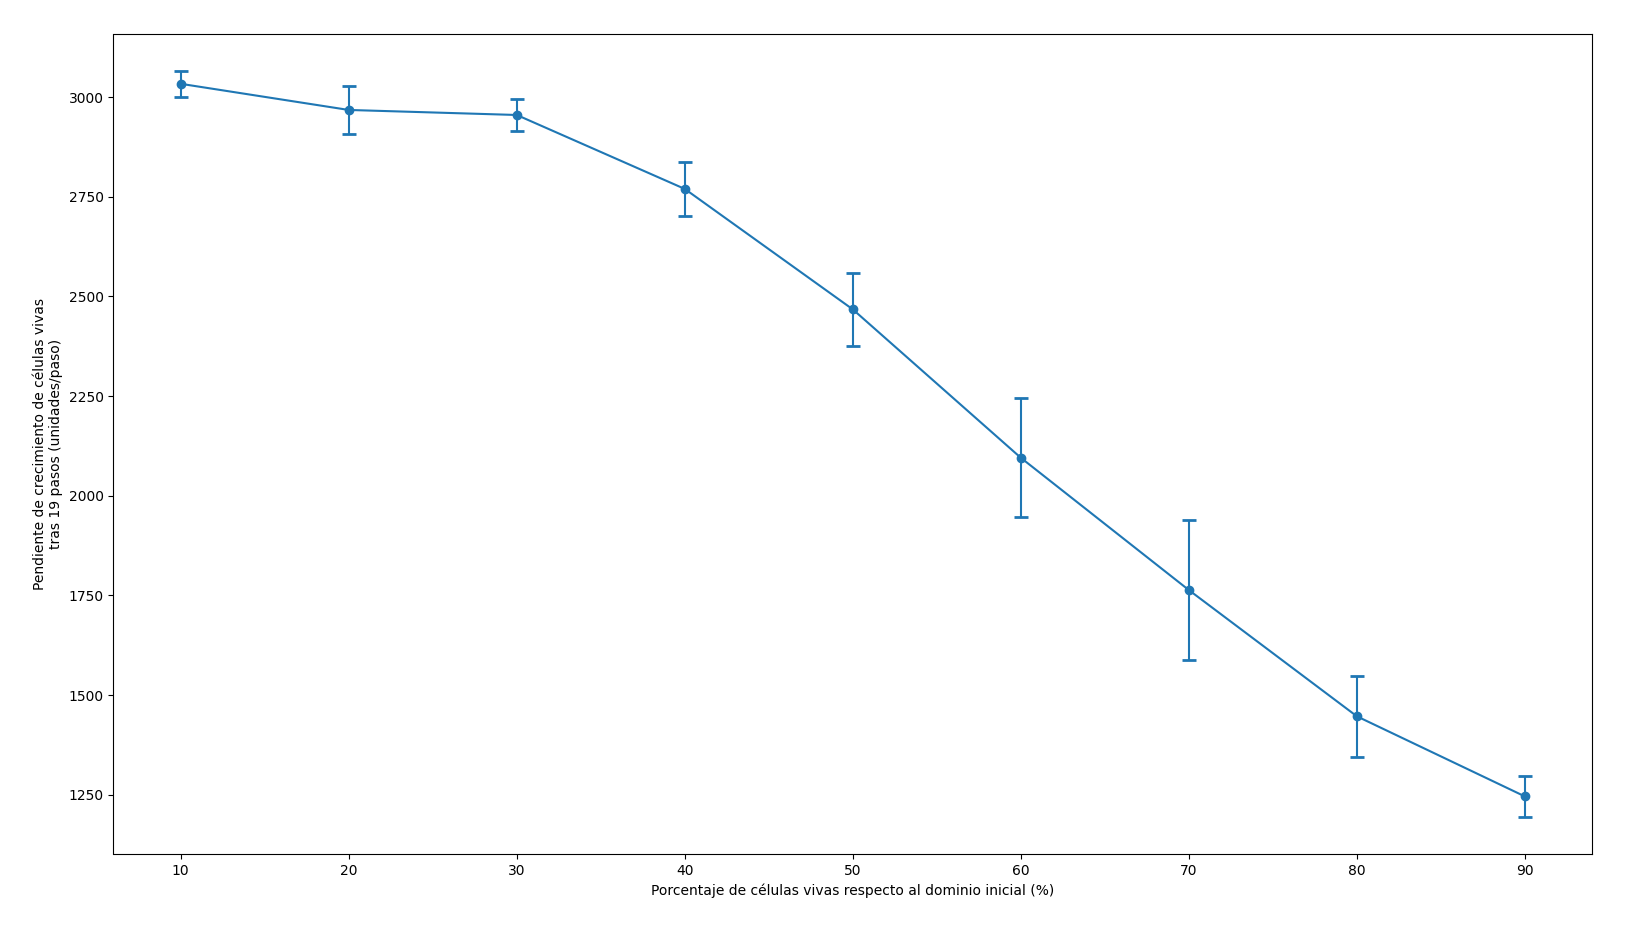
\includegraphics[width=0.8\linewidth]{pic/cubo3d/observable}
        \label{fig:expcub:size}
    \end{figure}
\end{frame}

